\documentclass[a4paper,14pt]{extarticle}
\usepackage[utf8]{inputenc}
\usepackage{amsmath}
\usepackage{amssymb}
\usepackage{fontspec}
\usepackage[T1]{fontenc}
\usepackage{caption}
\usepackage{hyperref}
\usepackage{array}
\usepackage{tabularx}
\usepackage{graphicx}
\usepackage{background} 
\backgroundsetup{contents=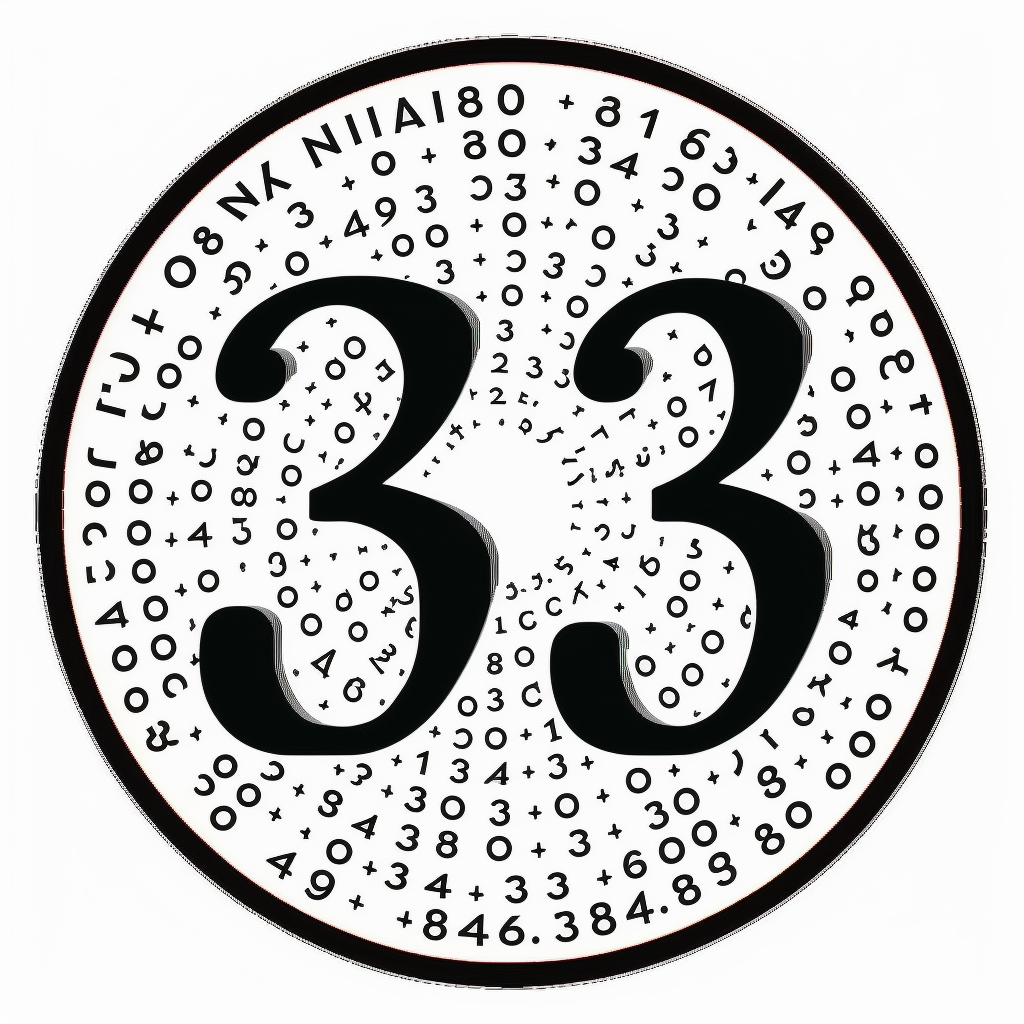
\includegraphics{static/logo.png}, opacity=0.1, scale=.3, angle=45d}
\title{\LARGE \textsf{Ptolemy's Theorem}}
\author{\textsf{Saugat Dhakal, Asal KC}}
\date{\textsf{27th Janurary, 2023}}
\begin{document}


\setsansfont{DMSans}[
    Path=./static/,
    Scale=0.9,
    Extension = .ttf,
    UprightFont=*-Regular
    ]
\maketitle
\section{\textsf{Introduction}}
    \textsf{Ptolemy, a Roman Mathematician, has made important contributions to the field of astrology, geography and mathematics. One of the more significant contributions made in the field of Mathematics by Ptolemy is the Ptolemy's Theorem.}
    \par
    \vspace{0.5cm}
    \textsf{Ptolemy's Theorem states that "In a cyclic quadrilateral, the product of the diagonals is equal to the sum of the product of the opposite sides of the cyclic quadrilateral."}
    \par
    \vspace{0.5cm}
    \textsf{Ptolemy's Theorem focuses on the relation between length of diagonals and edges of the cyclic quadrilateral. Cyclic quadrilateral is the special type of quadrilateral which is inscribable inside a circle. Now, there are multiple proofs available of the Ptolemy's Theorem. But, we are going to prove this theorem in basic plane geometry by using property of similarity of triangles.}
    \par
    \vspace{1cm}
    {\textsf{PROOF:}}
    \par 
    \vspace{.5cm}
    \textsf{In the given figure, ABCD is a cyclic quadrilateral inscribed in a circle with centre at O. 
    \begin{figure}[htp]
    \centering
    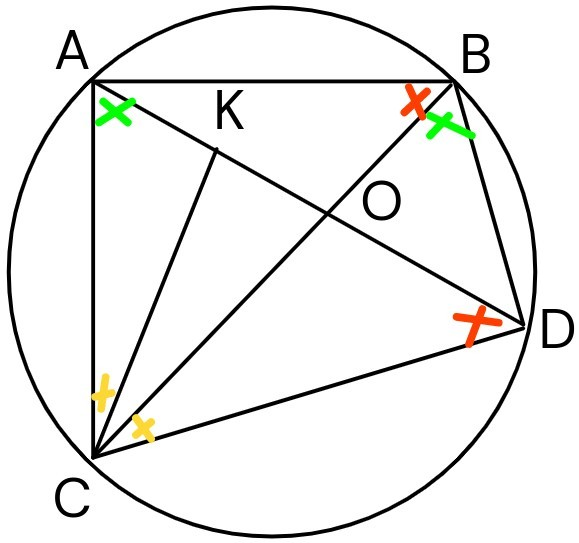
\includegraphics[width=6cm]{static/Studio_Project.jpeg}
    \caption{}
    \label{fig:galaxy}
\end{figure}
    We know,} \\ \\
    1. $\angle$ CAD = $\angle$ CBD (angles on same segment) ... (1) \\
    2. $\angle$ ABC = $\angle$ ADC (angles on same segment) ... (2) \\ \\
    \textsf{Now, construct a line from C meeting K at the diagonal AD such that} \\ 
    1. $\angle$ ACK = $\angle$ BCD (by construction) ... (1) \\ \\
    \textsf{then, } \\  
    In $\triangle$ ACK and $\triangle$ BCD, \\
    1. $\angle$ ACK = $\angle$ BCD (from equation 3) \\
    2. $\angle$ KAC = $\angle$ DBC (from equation 1) \\
    3. $\angle$ CKA = $\angle$ CDB (remaining angles of a triangle) \\ \\
    \textsf{then, } 
    $\triangle$ ACK $\sim$ $\triangle$ BCD \\
    \textsf{So, } 
    $\frac{AC}{BC}$ = $\frac{CK}{CD}$ = $\frac{AK}{BD}$ \textsf{(corresponding sides of a similar triangle are proportional)} \\
    $\Rightarrow$ AC.BD = BC.AK ... (4) \\ \\
    \textsf{again, }\\ \\
    In $\triangle$ ABC and $\triangle$ CDK, \\
    1. $\angle$ ABC = $\angle$ CDK (from equation 2) \\
    2. $\angle$ BCA = $\angle$ KCD (from equation 3) (adding $\angle$ KCO to both sides) \\
    3. $\angle$ CAB = $\angle$ DKC (remaining angles of a triangle) \\ \\
    \textsf{then, } 
    $\triangle$ ABC $\sim$ $\triangle$ CDK \\
    \textsf{So, } 
    $\frac{AB}{KD}$ = $\frac{BC}{CD}$ = $\frac{AC}{CK}$ \textsf{(corresponding sides of a similar triangle are proportional)} \\
    $\Rightarrow$ AB.CD = BC.KD ... (5) \\ \\
    \textsf{Adding equation 4 and 5, we obtain, \\}
    AC.BD + AB.CD = BC.KD + BC.AK \\
    $\Rightarrow$ AC.BD + AB.CD = BC.(KD + AK) \\
    $\Rightarrow$ AC.BD + AB.CD = BC.AD \\ \\
    \textsf{Thus, the theorem is proved. }
\end{document}
